\documentclass[12pt]{article}
\usepackage[margin=2cm]{geometry} 
\usepackage{titling}
\usepackage{graphicx}
\usepackage{float}
\usepackage[hidelinks]{hyperref}
\usepackage[italian]{babel}

\setlength\parindent{0pt}
\setlength{\parskip}{1em}
\setlength{\droptitle}{-2cm}

\title{Istruzioni d'uso Thymio}
\author{Università della Svizzera Italiana}
\date{Versione \today \ (Thymio Suite 2.3.2)}


\begin{document}
\maketitle
\tableofcontents
\newpage


\section{Installazione}\label{installation}

\subsection{Windows}

Recarsi all'indirizzo \url{https://www.thymio.org/download-thymio-suite-redirect} e scaricare il software Thymio Suite cliccando sul bottone \texttt{Download} sotto il logo Windows. Prestare attenzione a scegliere la versione adatta al proprio sistema (32/64 bit).\\
Aprire il file .exe scaricato e proseguire con l'installazione guidata. Al primo avvio dell'applicazione potrebbe essere necessario autorizzarla ad accedere a internet: cliccare su "Consenti accesso" nella finestra di dialogo di Windows Firewall.

\subsection{MacOS}

Recarsi all'indirizzo \url{https://www.thymio.org/download-thymio-suite-redirect} e scaricare il software Thymio Suite cliccando sul bottone \texttt{Download} sotto il logo Apple.\\
Aprire il file .dmg scaricato e trascinare il file ThymioSuite.app in Applicazioni.

\subsection{Linux}

Di seguito sono riportate le indicazioni per Ubuntu a partire dalla versione 18.04. Per altre distribuzioni, consultare la relativa documentazione ufficiale.

1. Installare \texttt{flatpak}, un sistema di distribuzione di applicazioni, se non già presente:

\texttt{sudo apt install flatpak}

\texttt{sudo apt install gnome-software-plugin-flatpak}

\texttt{flatpak remote-add --if-not-exists flathub https://flathub.org/repo/flathub.flatpakrepo}

Riavviare il computer.

2. Configurare le porte per la connessione:

\texttt{sudo nano /etc/udev/rules.d/99-mobsya.rules}

Aggiungere le seguenti due linee:

\texttt{SUBSYSTEM=="usb", ATTRS\{idVendor\}=="0617", ATTRS\{idProduct\}=="000a", MODE="0666"}\\
\texttt{SUBSYSTEM=="usb", ATTRS\{idVendor\}=="0617", ATTRS\{idProduct\}=="000c", MODE="0666"}

Salvare e uscire (CTRL+O, Enter,  CTRL+X).

\texttt{sudo udevadm control --reload-rules}


3. Installare Thymio Suite:

\texttt{flatpak install flathub org.mobsya.ThymioSuite}\\


Documentazione ufficiale: \url{https://www.thymio.org/linux-installation}


\section{Collegamento del robot}

Prima di utilizzare qualsiasi software, è necessario collegare almeno un robot al computer (vedi sezione \ref{multi-robot} per multipli robot). Questo può essere fatto in due modi: tramite cavo o wireless (se supportato).

\subsection{Cavo USB}

Collegare il cavo in dotazione ad una porta libera sulla propria macchina e alla porta microUSB sul retro del Thymio. Il robot si accenderà automaticamente non appena rilevata la connessione.

\subsection{Dongle wireless (se disponibile)}

Collegare il dongle ad una porta libera sulla propria macchina e accendere il robot tenendo premuto il tasto centrale per circa 3 secondi. Il LED del dongle e del robot dovrebbero lampeggiare alla stessa frequenza.

\newpage

\section{Software}

Tutti i programmi necessari per configurare e programmare Thymio sono raccolti in una sola applicazione, Thymio Suite.

\begin{figure}[H]
	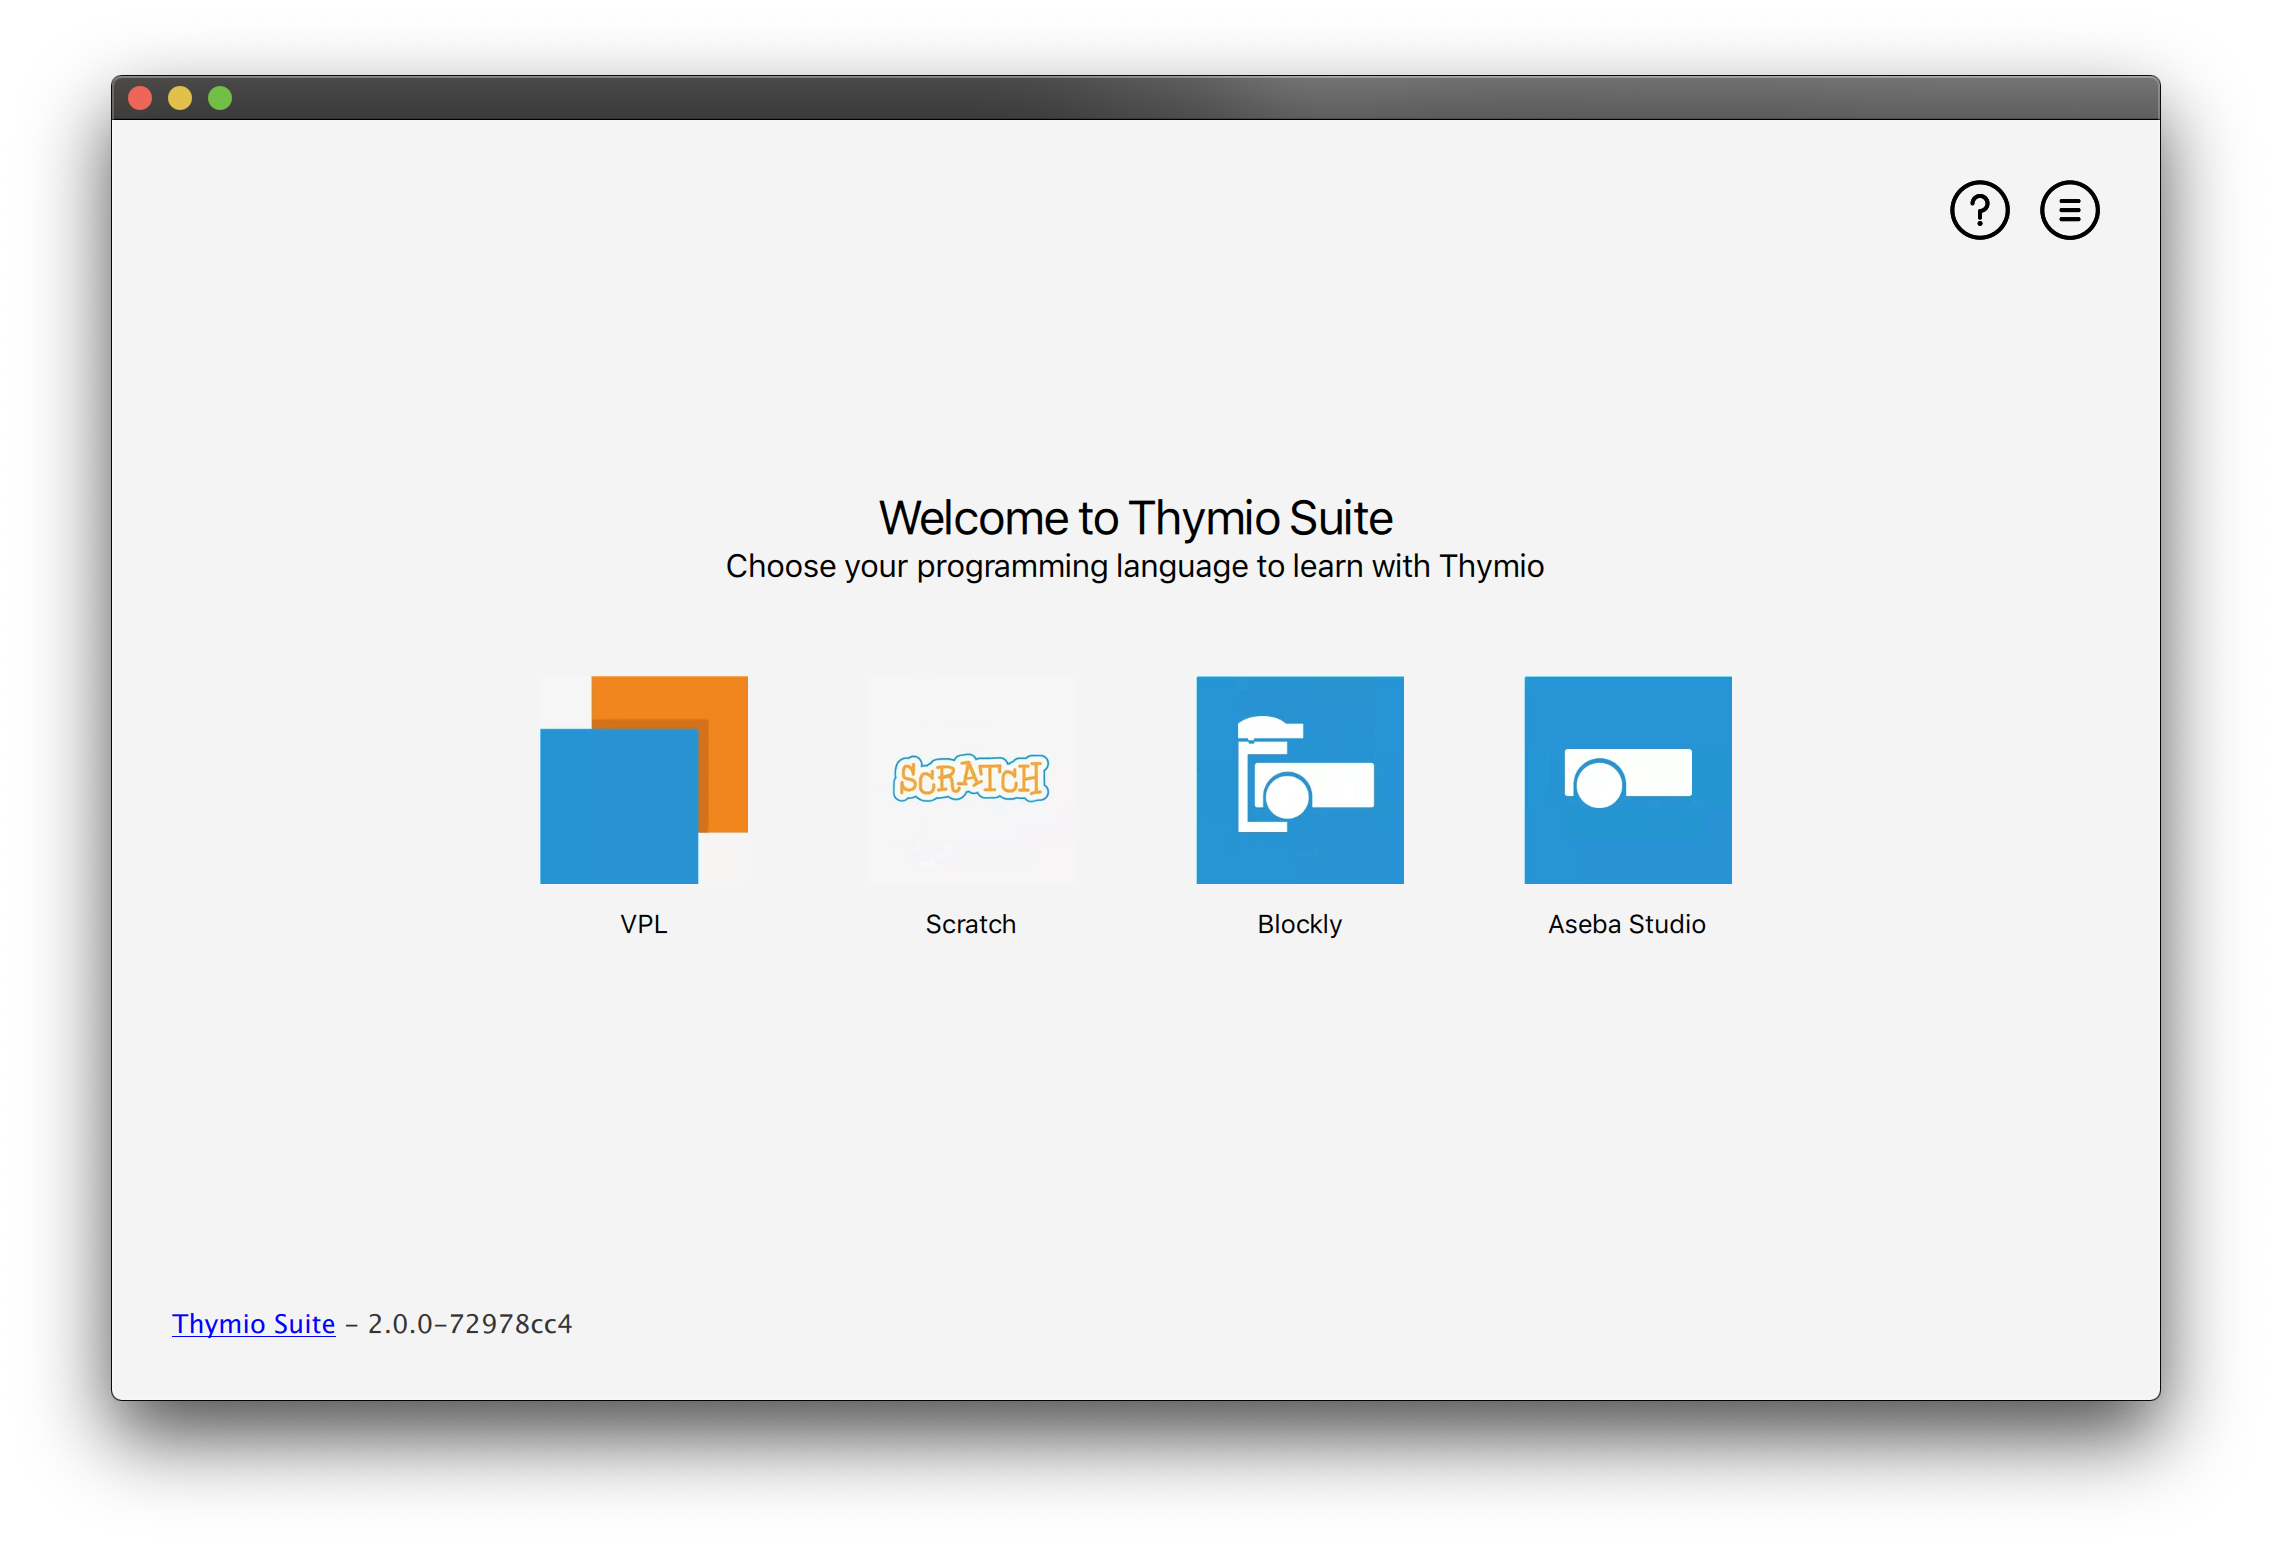
\includegraphics[width=\textwidth]{img/thymioSuite.png}
	\caption{La finestra principale di Thymio Suite}
	\label{aseba1}
\end{figure}

Nota: in caso Blockly, VPL e Scratch non dovessero aprirsi al click della relativa icona, recarsi nel menu a destra e deselezionare la casella \texttt{Utilizzare il browser predefinito del sistema}.

\newpage

Nota: su MacOS è possibile che il programma sia bloccato dal sistema siccome proviene da una fonte esterna (vedi figura \ref{macErr}). Cliccare su Annulla, in seguito recarsi in Impostazioni di Sistema, sotto Sicurezza e Privacy e cliccare su Apri Comunque. Ora è possibile avviare il software, cliccando un'ultima volta su Apri quando richiesto. Altri avvisi appariranno lanciando Blockly e le altre applicazioni, ma sarà sufficiente cliccare su Apri.

\begin{figure}[H]
	\centering
	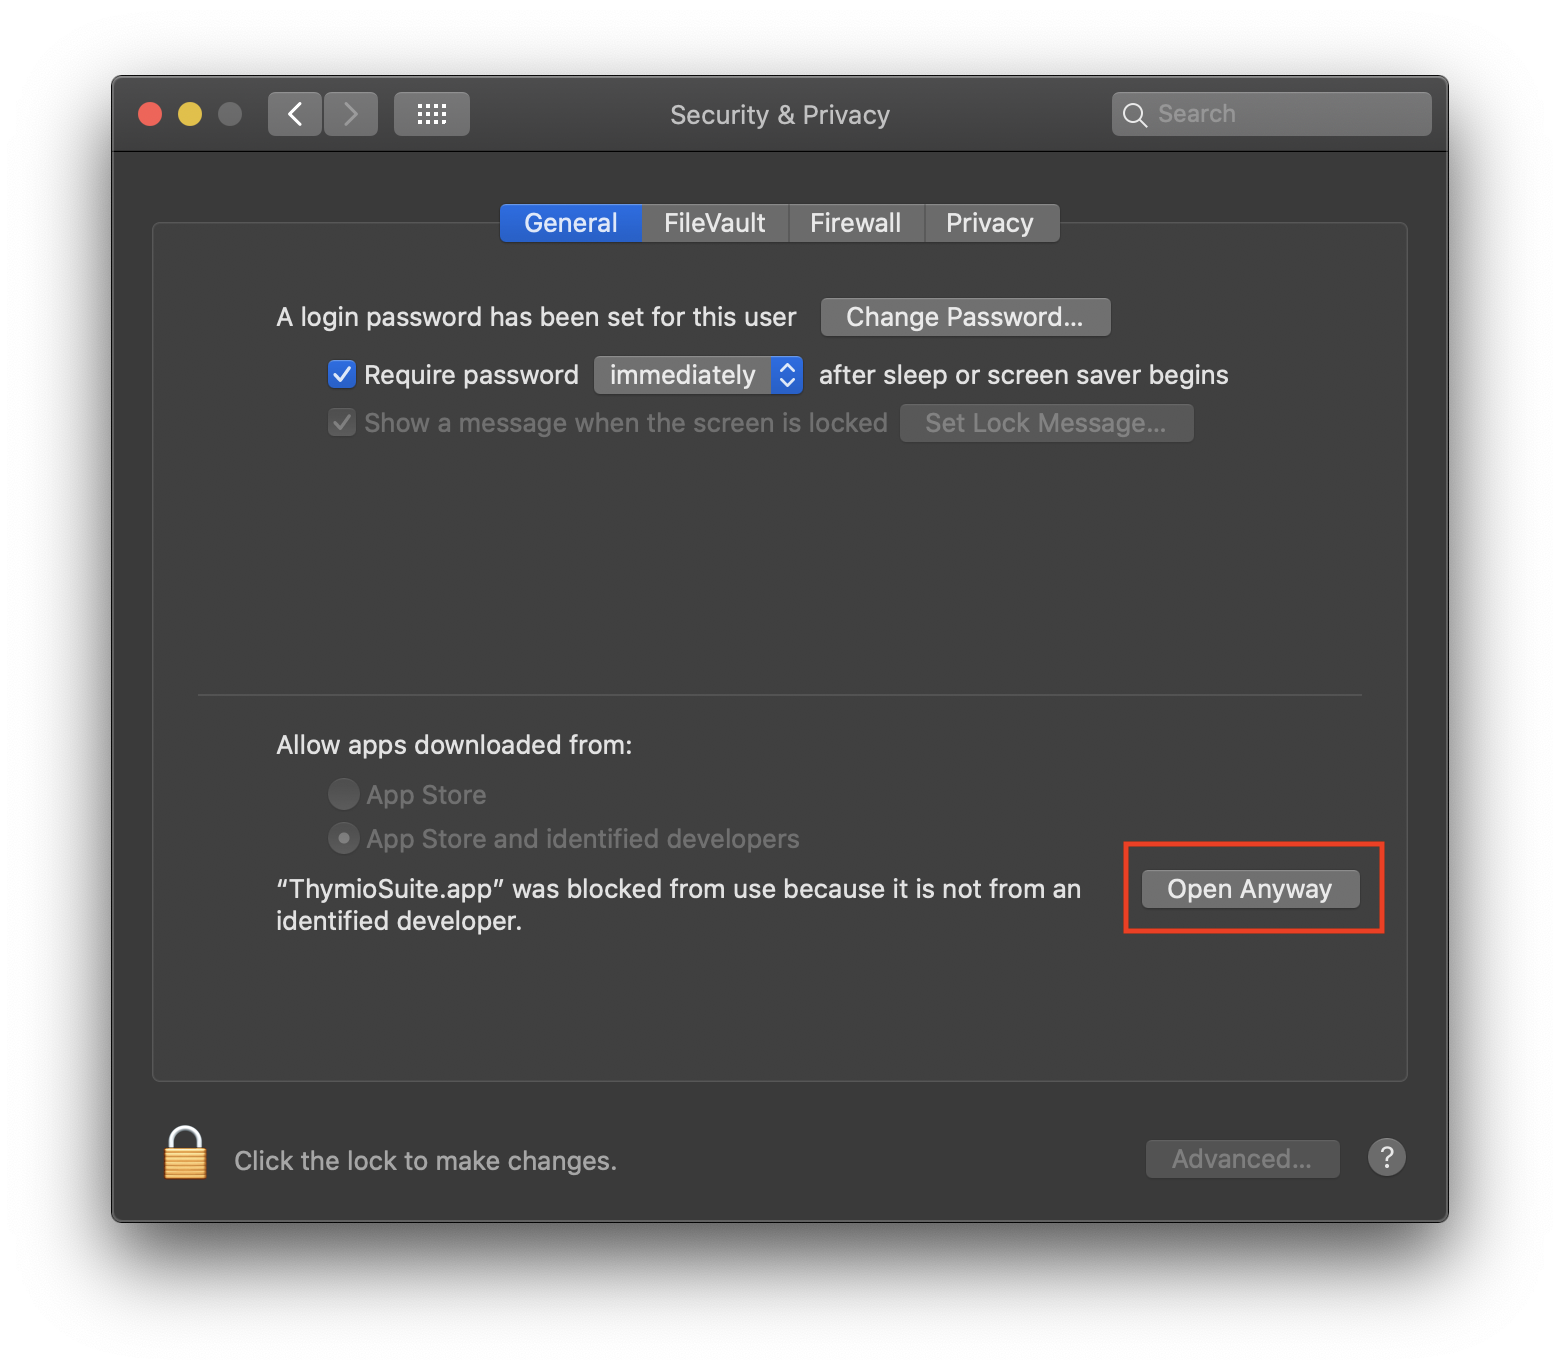
\includegraphics[width=0.7\textwidth]{img/macWarn.png}
	\caption{Le Impostazioni di Sistema di MacOS}
	\label{macErr}
\end{figure}

\newpage

\subsection{Aseba Studio}

Aseba Studio è un software per programmare direttamente i robot Thymio, pensato per utenti più esperti. Per utilizzarlo è sufficiente lanciare Thymio Suite, cliccare sull'icona Aseba Studio e fare doppio click sul robot da programmare.

Nota: i file prodotti da Aseba Studio (in formato \texttt{.aesl}) possono essere aperti solo con questo software; inoltre, esso è in grado di aprire file salvati con Blockly e VPL (in formato \texttt{.aesl}), ma non con Scratch (in formato \texttt{.sb3}).

\begin{figure}[H]
	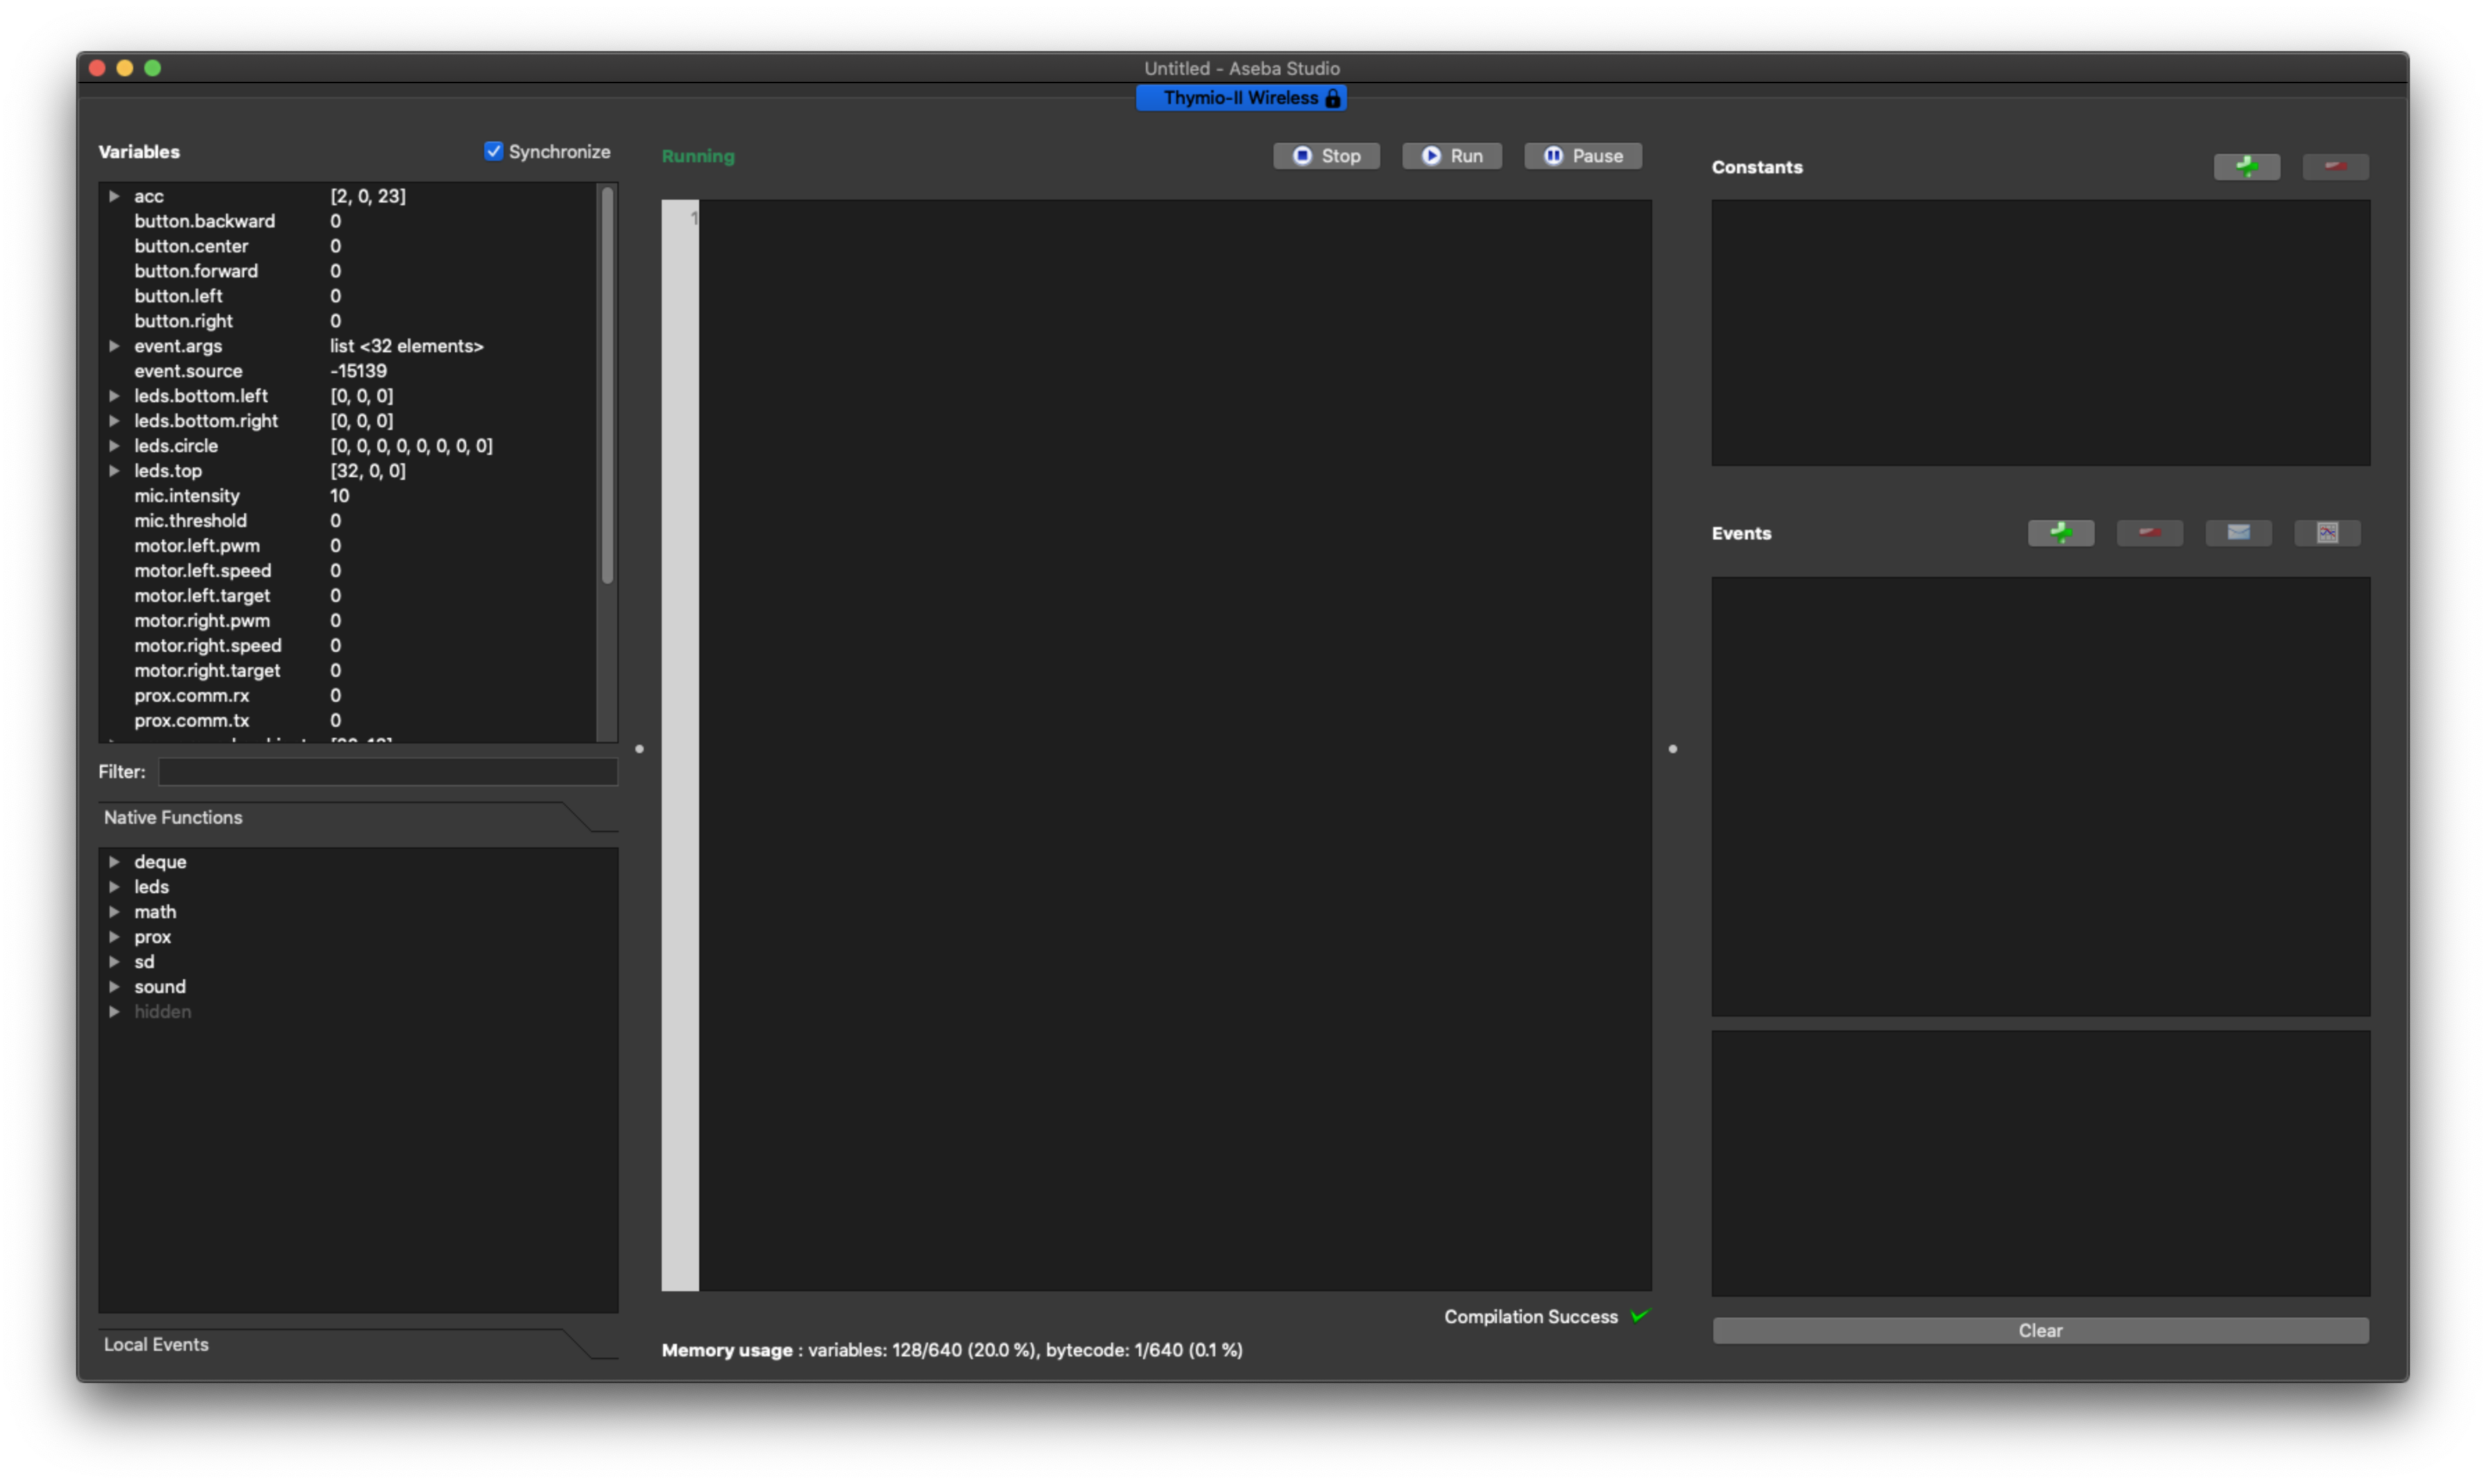
\includegraphics[width=\textwidth]{img/asebaStudio.png}
	\caption{La finestra principale di Aseba Studio}
	\label{main_aseba}
\end{figure}

\newpage

\subsection{Blockly}

Blockly è un software per programmare in maniera intuitiva. Per utilizzarlo è sufficiente lanciare Thymio Suite, cliccare sull'icona Blockly e fare doppio click sul robot da programmare.

Tramite l'icona di salvataggio è possibile esportare il proprio lavoro, che sarà possibile importare successivamente in Blockly o Aseba Studio.

\begin{figure}[H]
	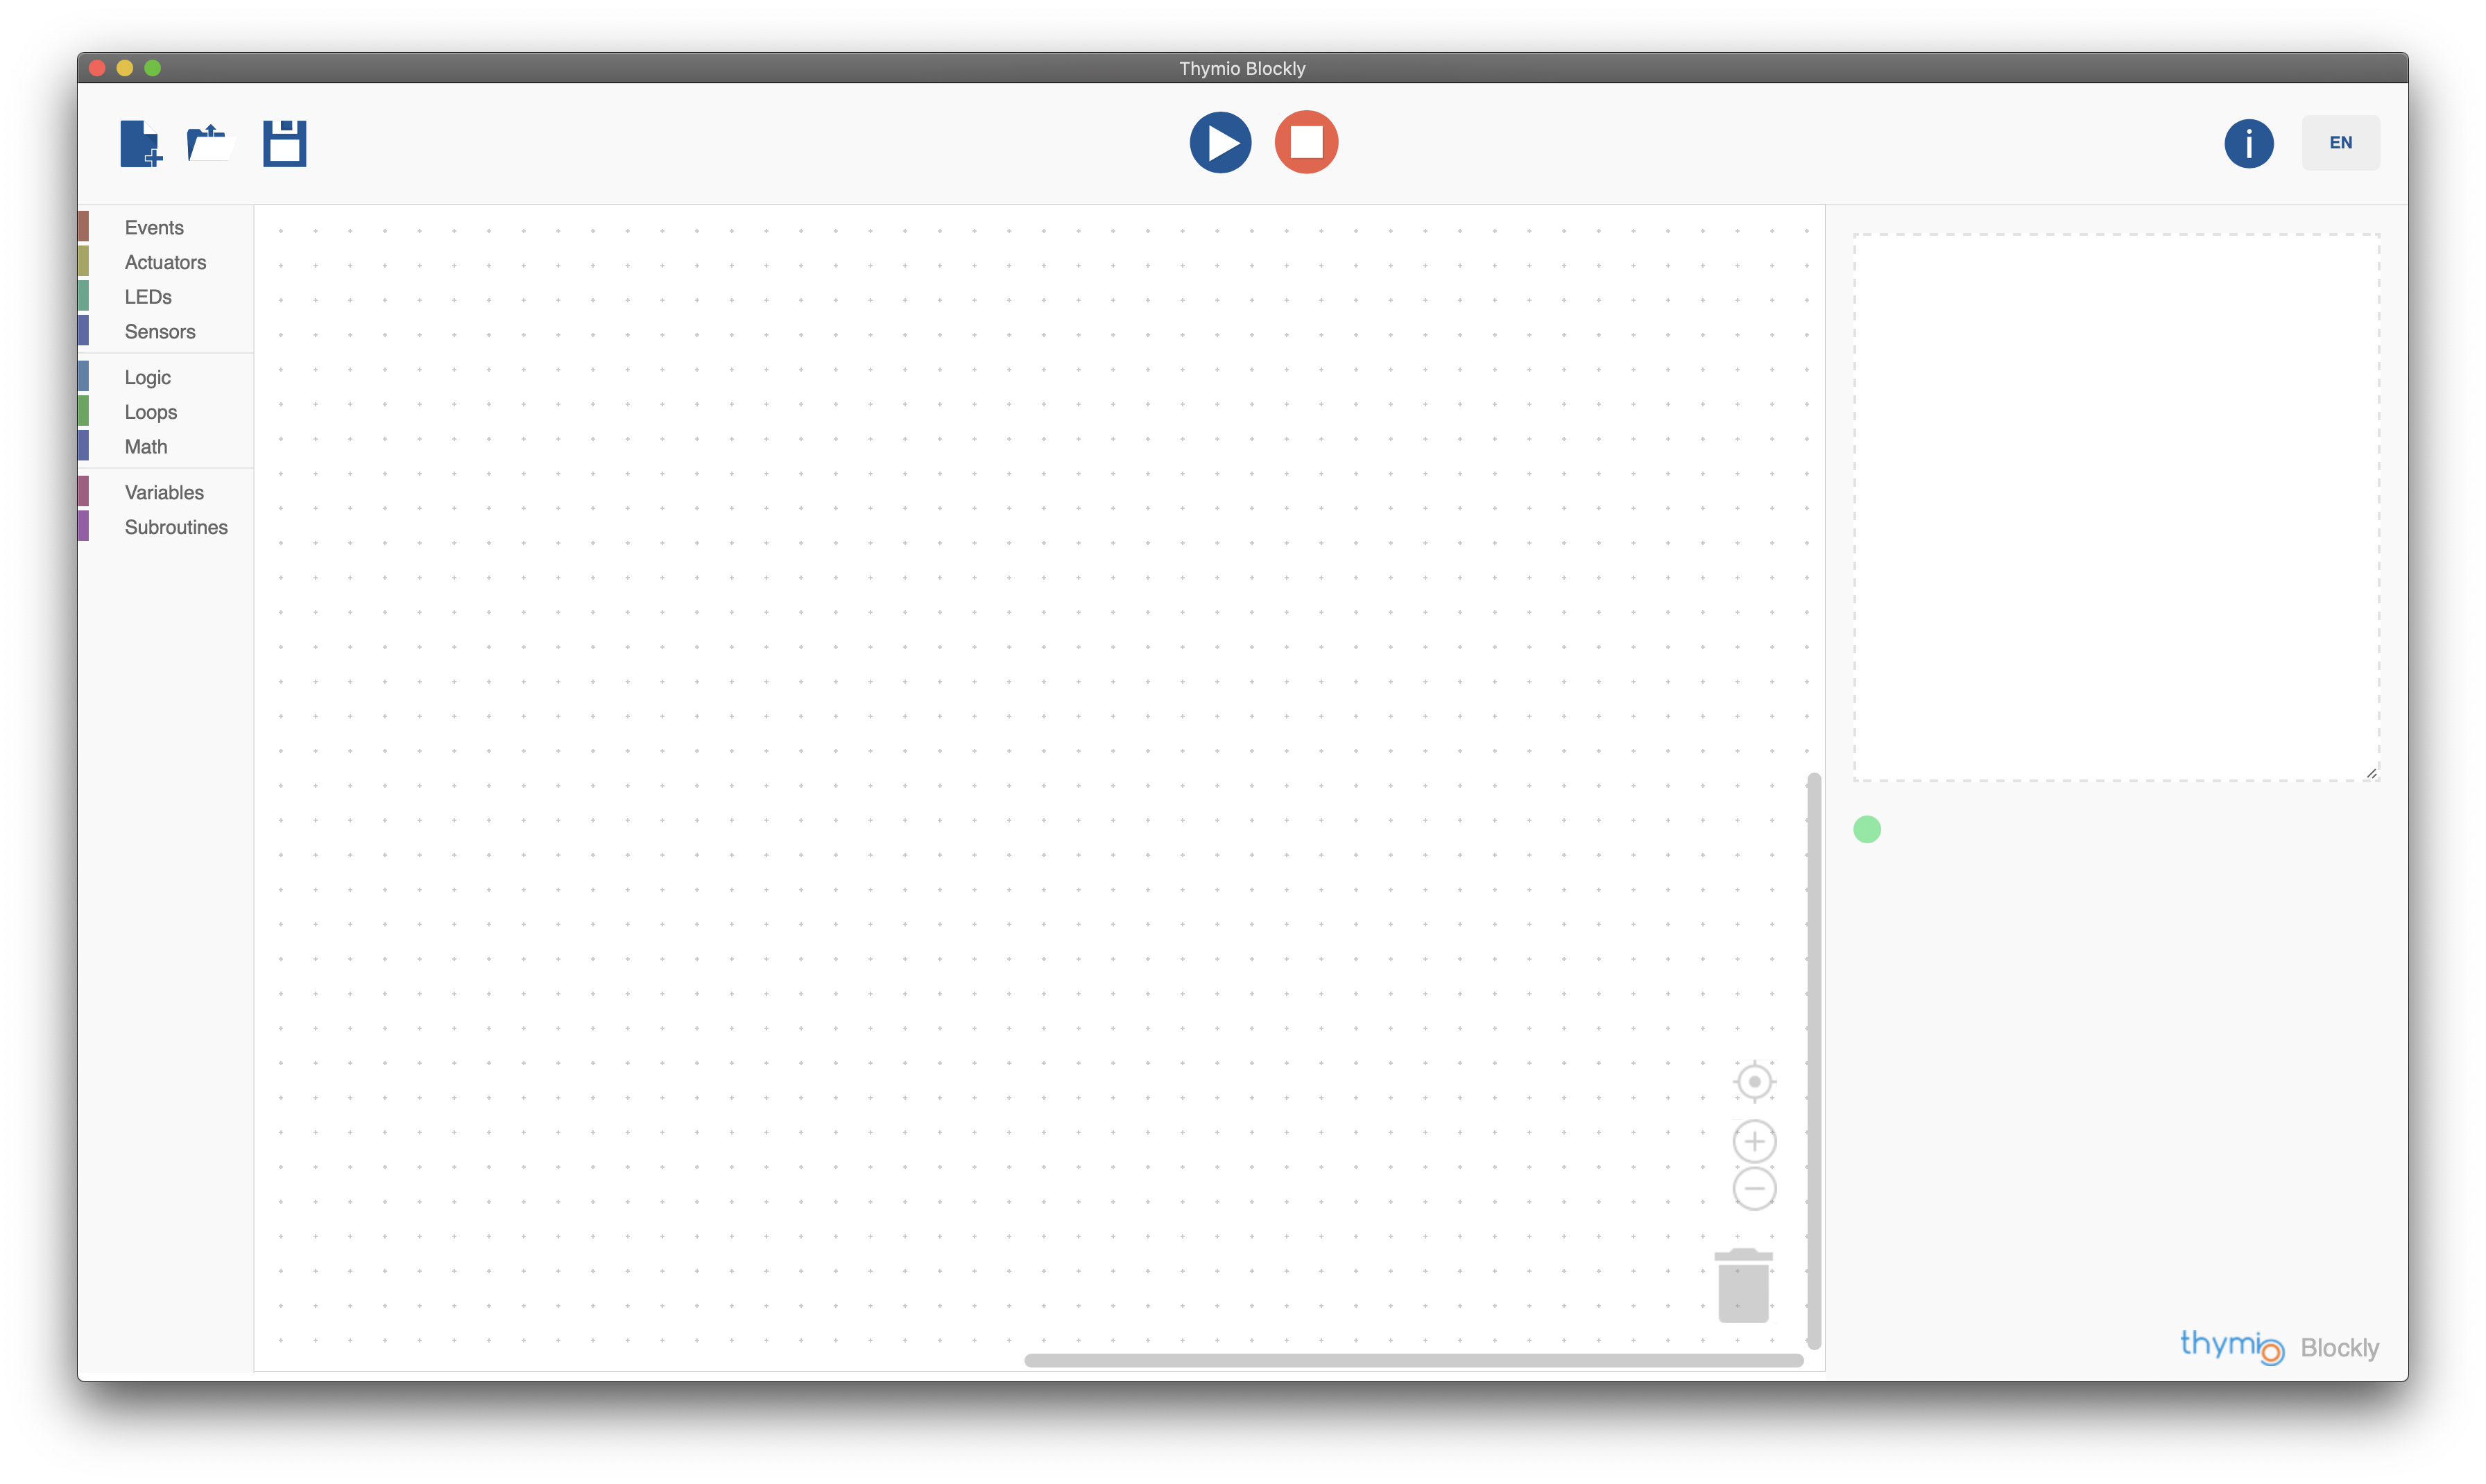
\includegraphics[width=\textwidth]{img/blockly.png}
	\caption{La finestra principale di Blockly}
	\label{main_blockly}
\end{figure}

\newpage

\subsection{VPL}

VPL (Visual Programming Language) è un software semplificato pensato per i più giovani. Per utilizzarlo è sufficiente lanciare Thymio Suite, cliccare sull'icona VPL e fare doppio click sul robot da programmare.

Tramite l'icona di salvataggio è possibile esportare il proprio lavoro, che sarà possibile importare successivamente in VPL o Aseba Studio.

\begin{figure}[H]
	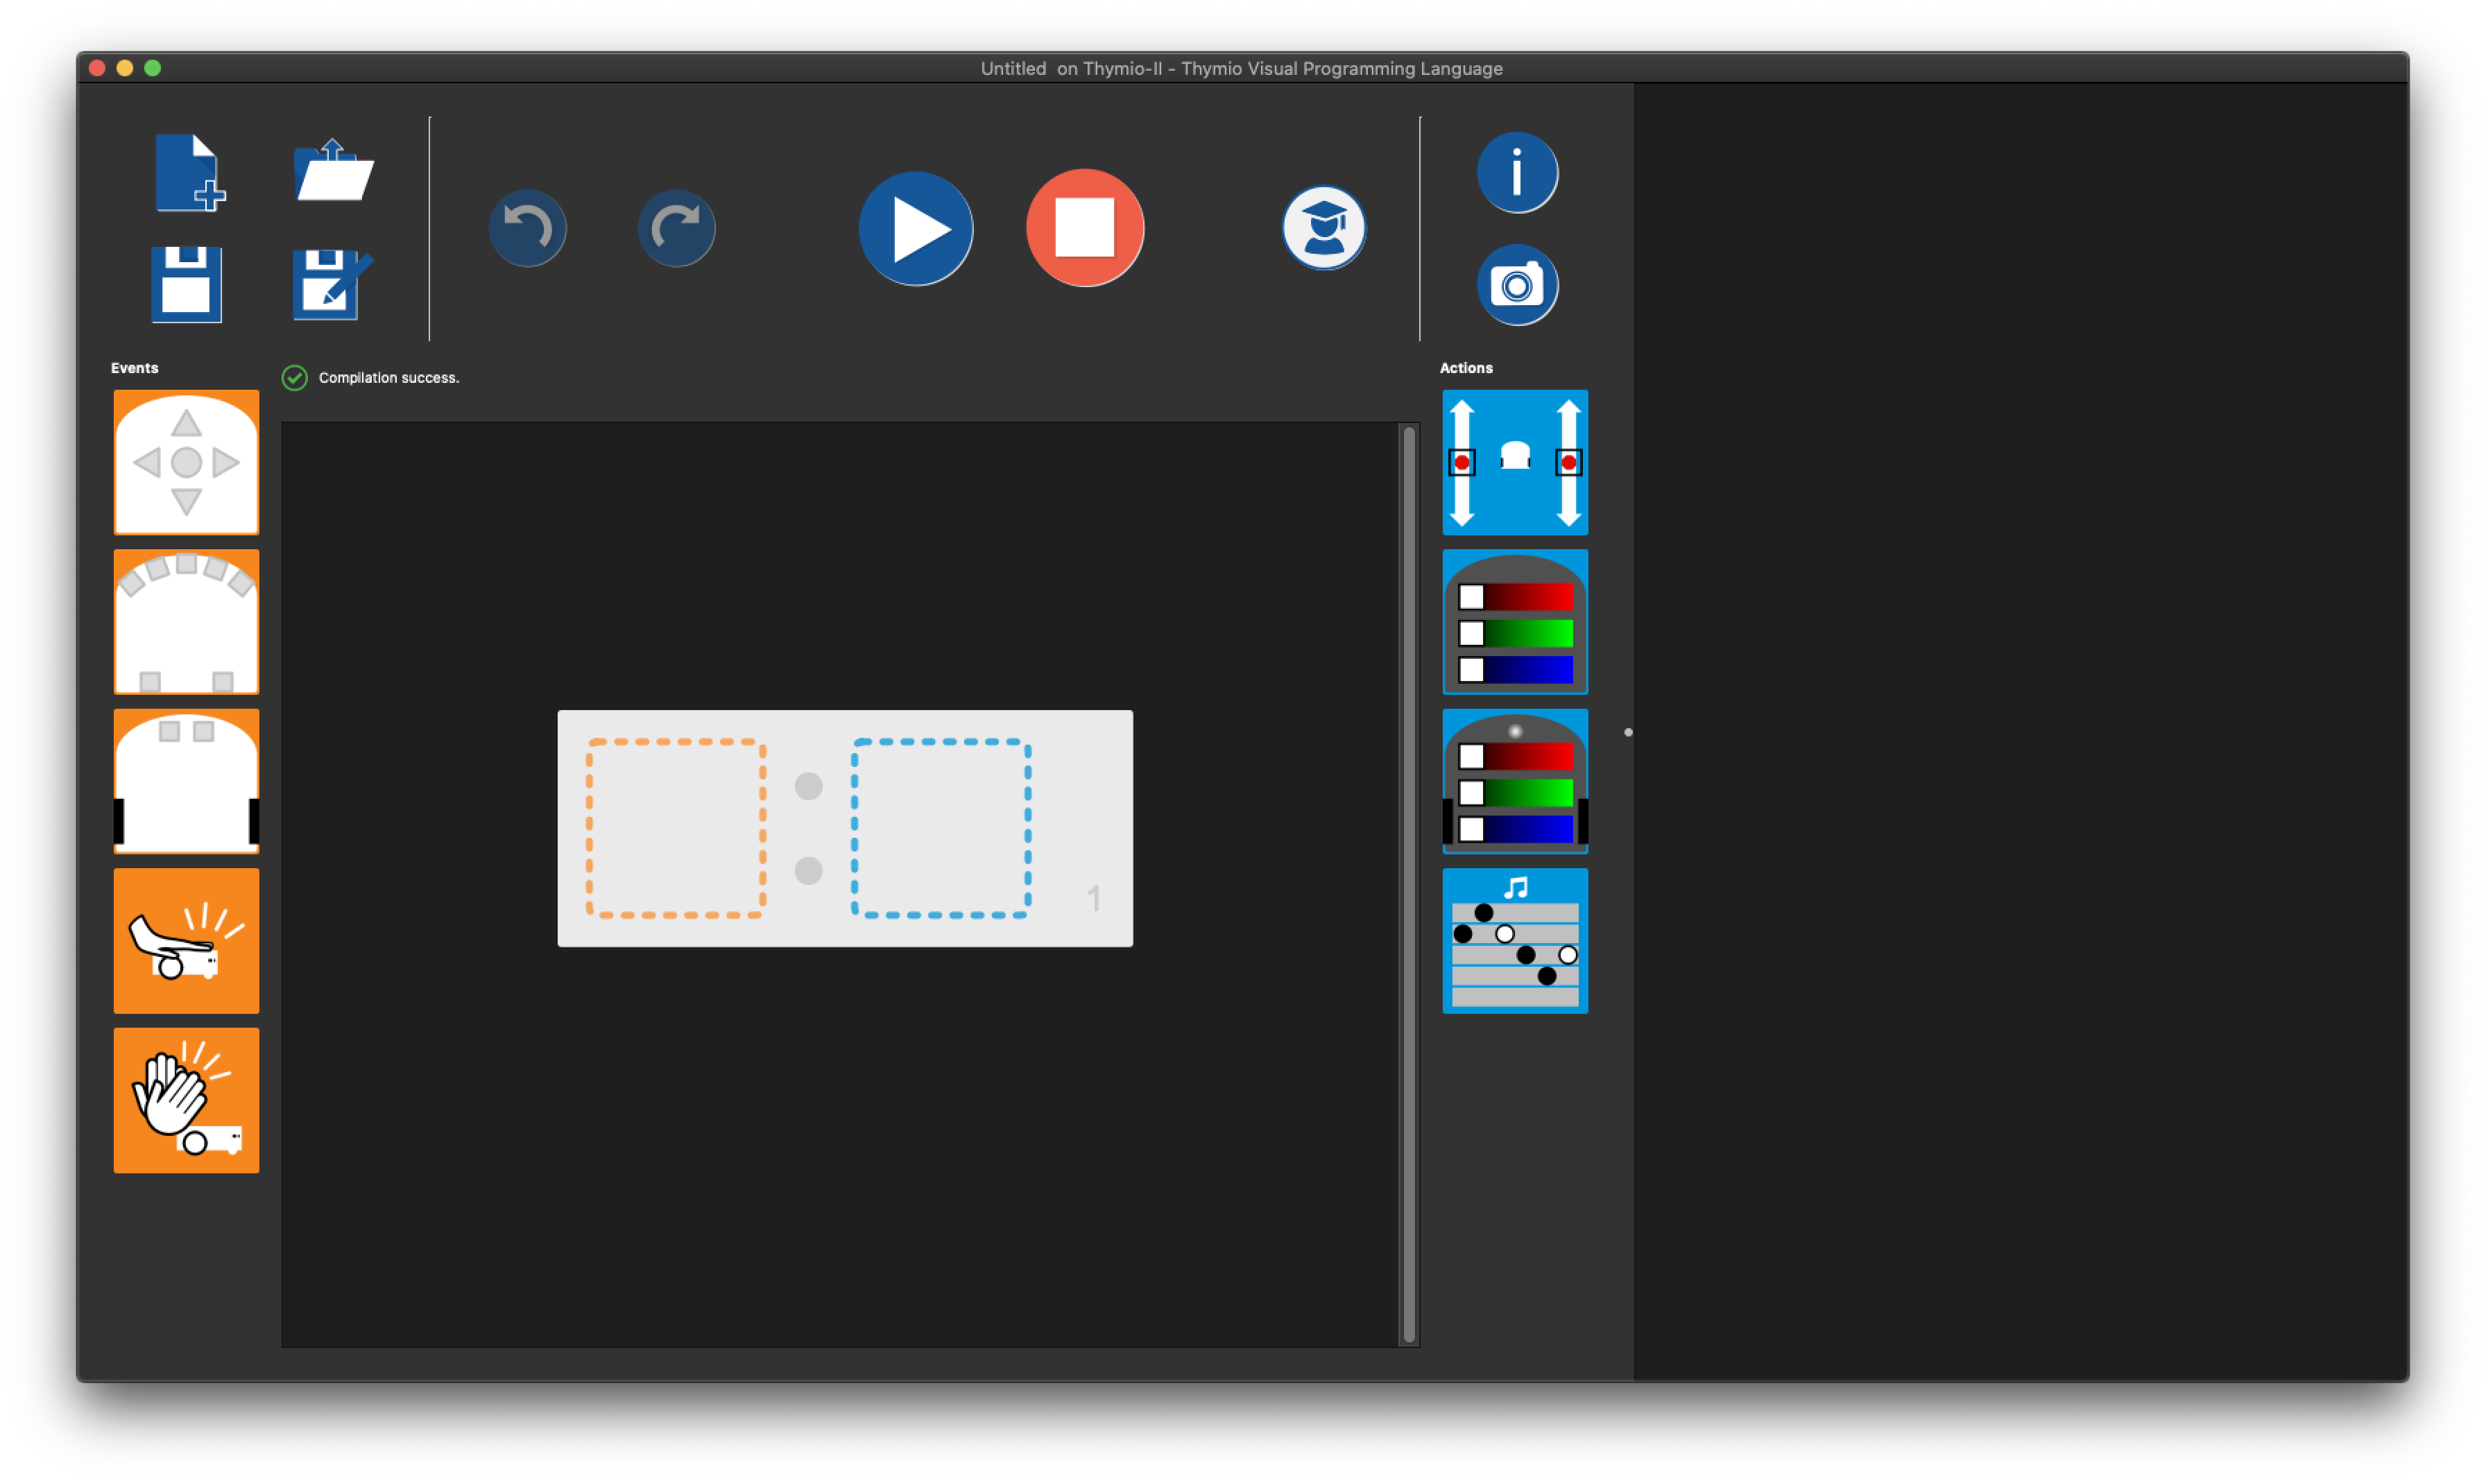
\includegraphics[width=\textwidth]{img/vpl.png}
	\caption{La finestra principale di VPL}
	\label{main_vpl}
\end{figure}

\newpage

\subsection{Scratch}

Scratch è un linguaggio educativo sviluppato dal MIT (sito ufficiale: \url{https://scratch.mit.edu}). Per utilizzarlo è sufficiente lanciare Thymio Suite, cliccare sull'icona Scratch e fare doppio click sul robot da programmare.

Tramite il menu \texttt{File} è possibile esportare il proprio lavoro, che sarà possibile importare successivamente in Scratch.

\begin{figure}[H]
	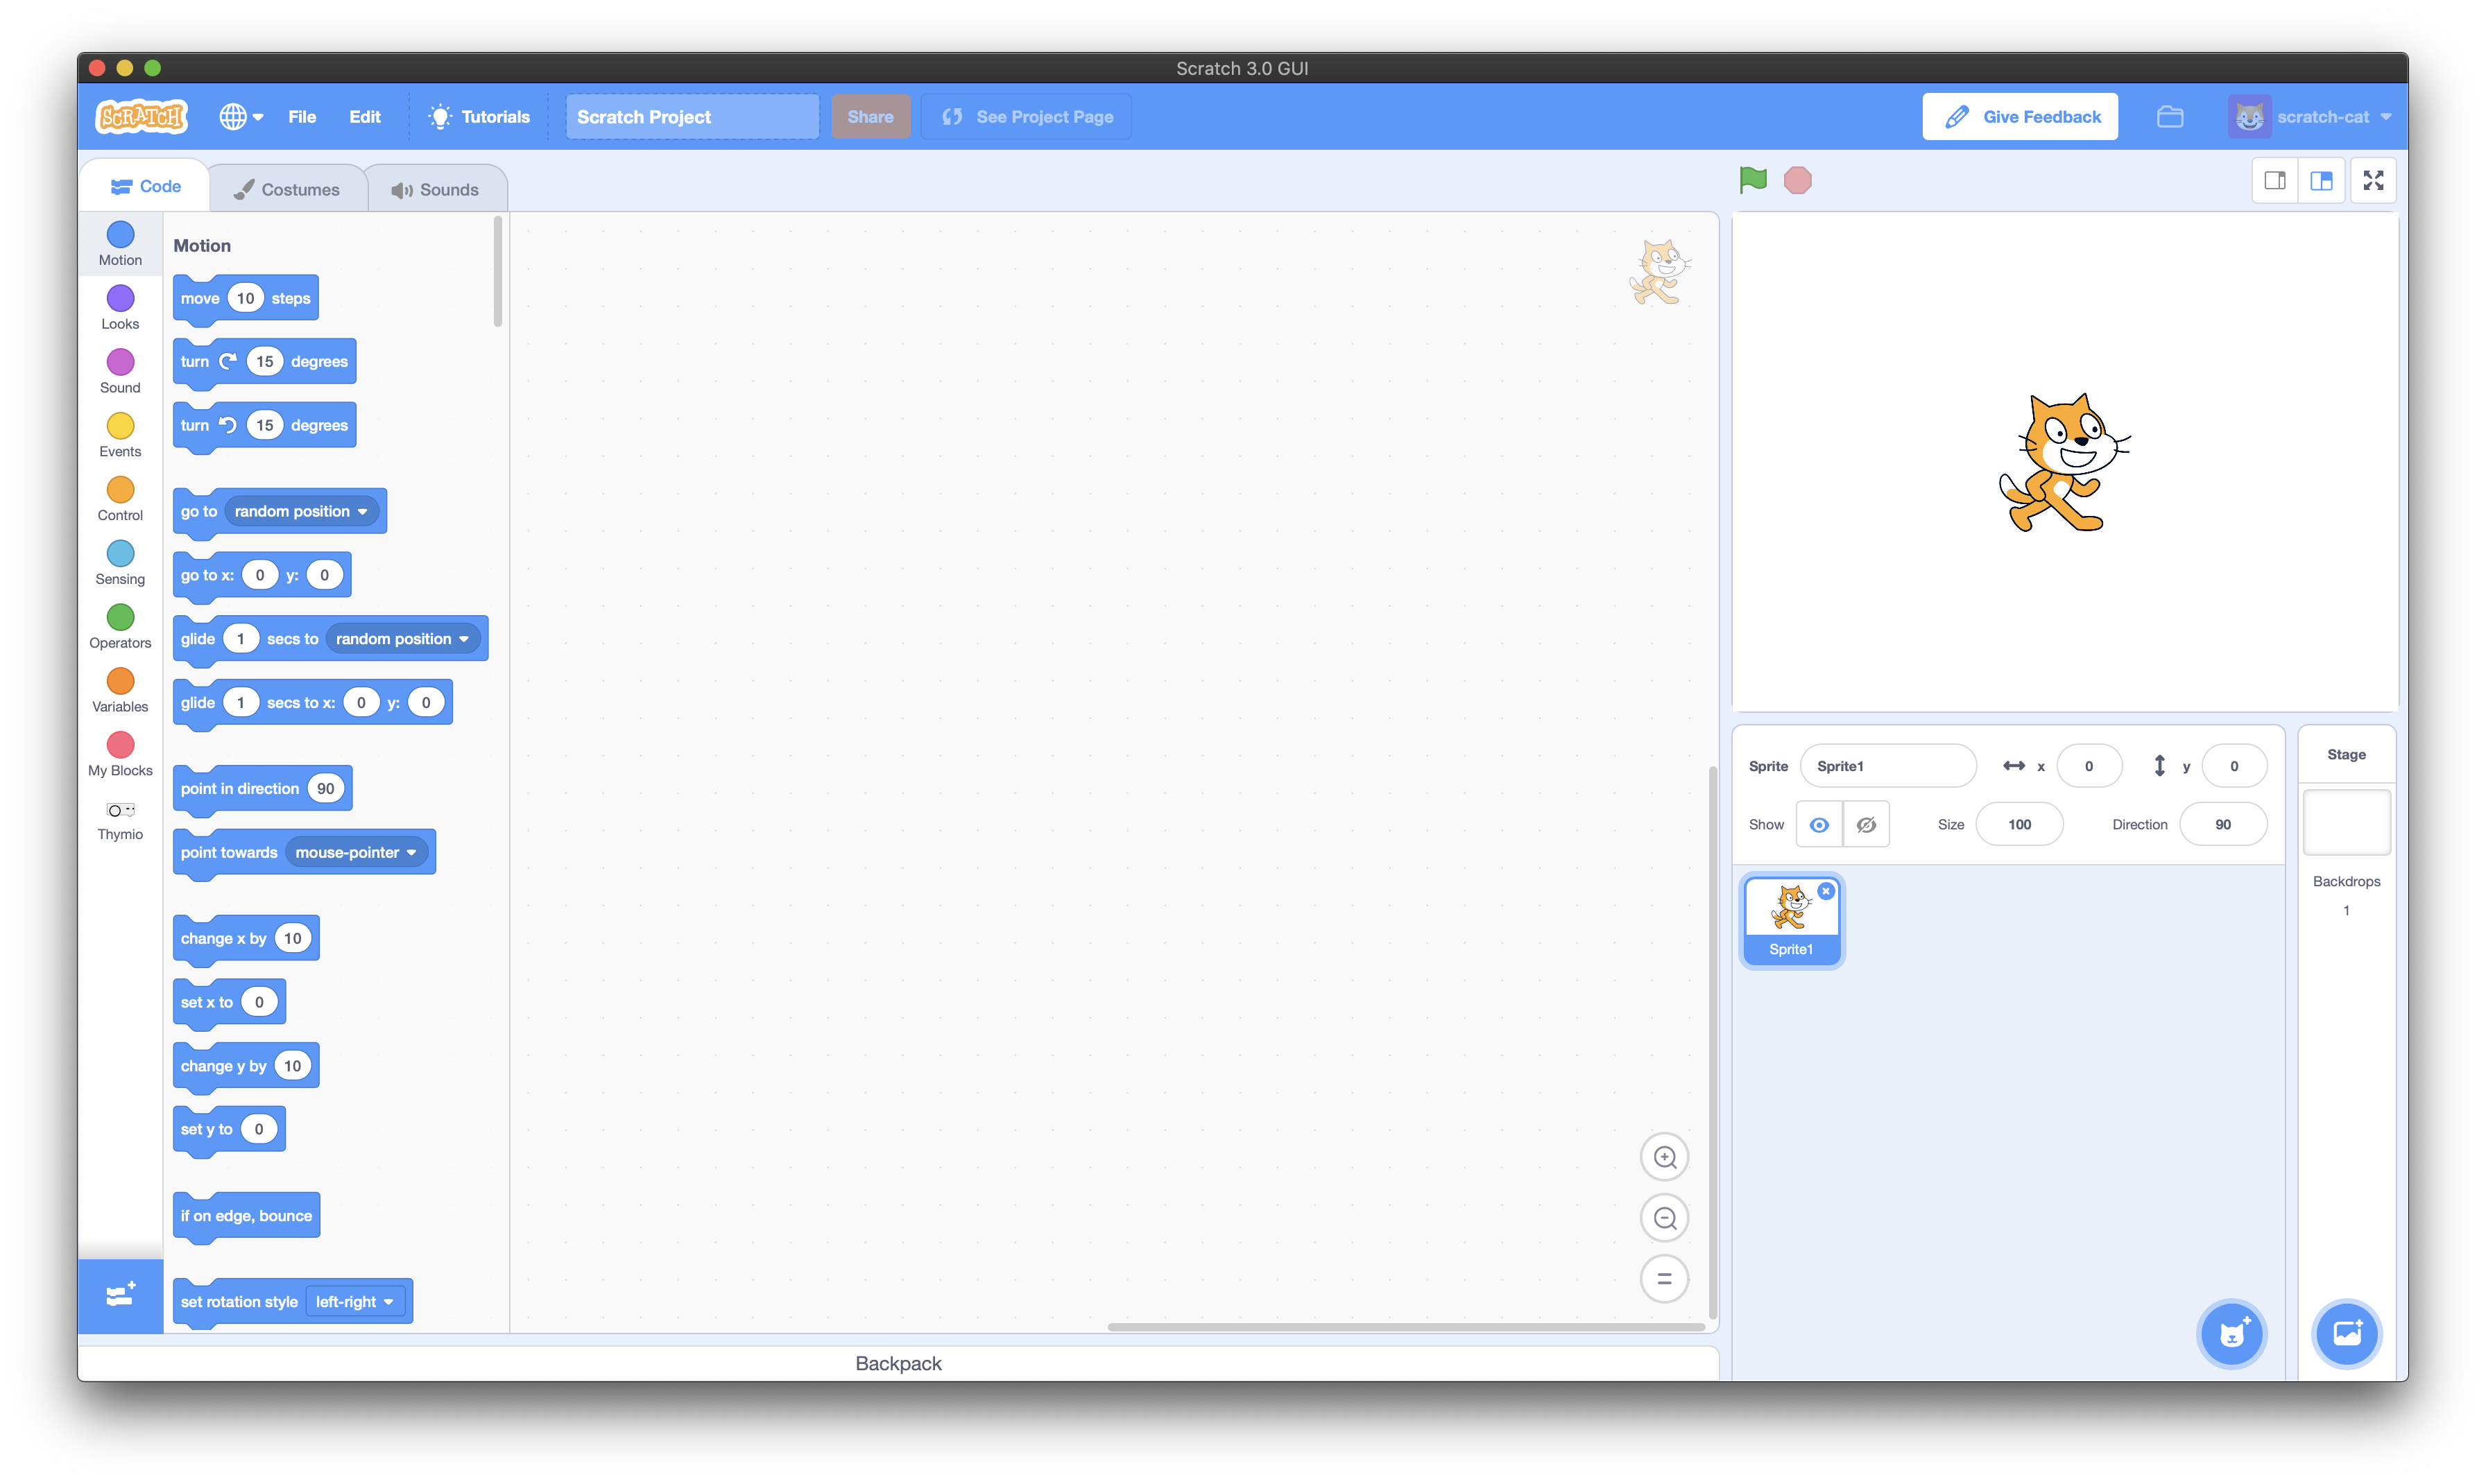
\includegraphics[width=\textwidth]{img/scratch.png}
	\caption{La finestra principale di Scratch}
	\label{main_scratch}
\end{figure}

\subsection{Thymio Simulator}

No Thymio? No problem! Esiste un simulatore previsto per emulare uno o più robot sul proprio computer, incluso direttamente nel pacchetto software scaricato al punto \ref{installation}.

Nota: su macOS e Linux, è necessario scaricare le mappe disponibili all'indirizzo \url{https://www.thymio.org/teaching-resources/simulator}.

Per utilizzarlo è sufficiente selezionare \texttt{Avviare il simulatore} dal menu a destra e scegliere la mappa desiderata; in seguito, selezionare il software di programmazione desiderato dall'applicazione principale.
I robot presenti nella simulazione saranno elencati come se fossero collegati al proprio computer e sarà possibile iniziare a programmarli.


\section{Aggiornamento del firmware}

Qualora un robot connesso dovesse avere un firmware non aggiornato, dopo aver selezionato il linguaggio di programmazione desiderato da Thymio Suite un'icona apparirà sul Thymio da aggiornare (vedi figura sottostante). Per iniziare l'aggiornamento è sufficiente cliccarla e confermare la scelta. Una barra blu indica lo stato dell'operazione.

\begin{figure}[H]
	\centering
	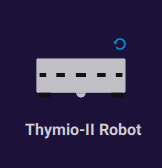
\includegraphics{img/fwUpgrade.png}
	\caption{Un robot con un firmware da aggiornare}
	\label{fwUpgrade}
\end{figure}

\textbf{NON} scollegare o spegnere il robot durante la procedura!

Video ufficiale illustrante la procedura completa: \url{https://youtu.be/-unIjKXrnUU}\\


\subsection{Installare un firmware specifico (utenti esperti)}

Qualora si volesse installare una versione specifica o personalizzata è necessario scaricare il vecchio pacchetto Aseba 1.6.1 disponibile al link riportato al punto \ref{installation}, sotto la voce \texttt{Scarica una versione precedente}.
Recarsi poi all'indirizzo \url{https://github.com/Mobsya/aseba-target-thymio2/releases} e scaricare il file \texttt{.hex} per la versione desiderata. Collegare il robot con il cavo USB e avviare Thymio Firmware Upgrader; scegliere Custom Firmware, selezionare il file appena scaricato e cliccare su Upgrade.

\textbf{NON} scollegare o spegnere il robot durante la procedura!

\newpage


\section{Collegare multipli robot}\label{multi-robot}

È possibile collegare diversi robot allo stesso computer e programmarli in maniera individuale, oppure definire degli eventi comuni. Un programma di esempio è disponibile all'indirizzo indicato al punto \ref{usiRepo} (remoteDrive).

Per fare ciò è necessario accoppiare tutti i robot desiderati con lo stesso dongle (se disponibile):

1. Collegare il dongle e il primo robot (tramite cavo USB) al proprio computer

2. Aprire Thymio Suite e dal menu a destra selezionare \texttt{Associa un wireless Thymio a un Wireless Dongle}

3. Cliccare su \texttt{Modalità avanzata} e scegliere un canale e un identificativo di rete (esadecimale)

4. Cliccare su \texttt{Associa!} e, dopo la conferma sonora, scollegare il robot

5. Collegare il prossimo, inserire lo stesso canale e identificativo scelti in precedenza

6. Ripetere i passaggi 4 e 5 per ogni altro robot che si desidera aggiungere alla rete


\begin{figure}[H]
	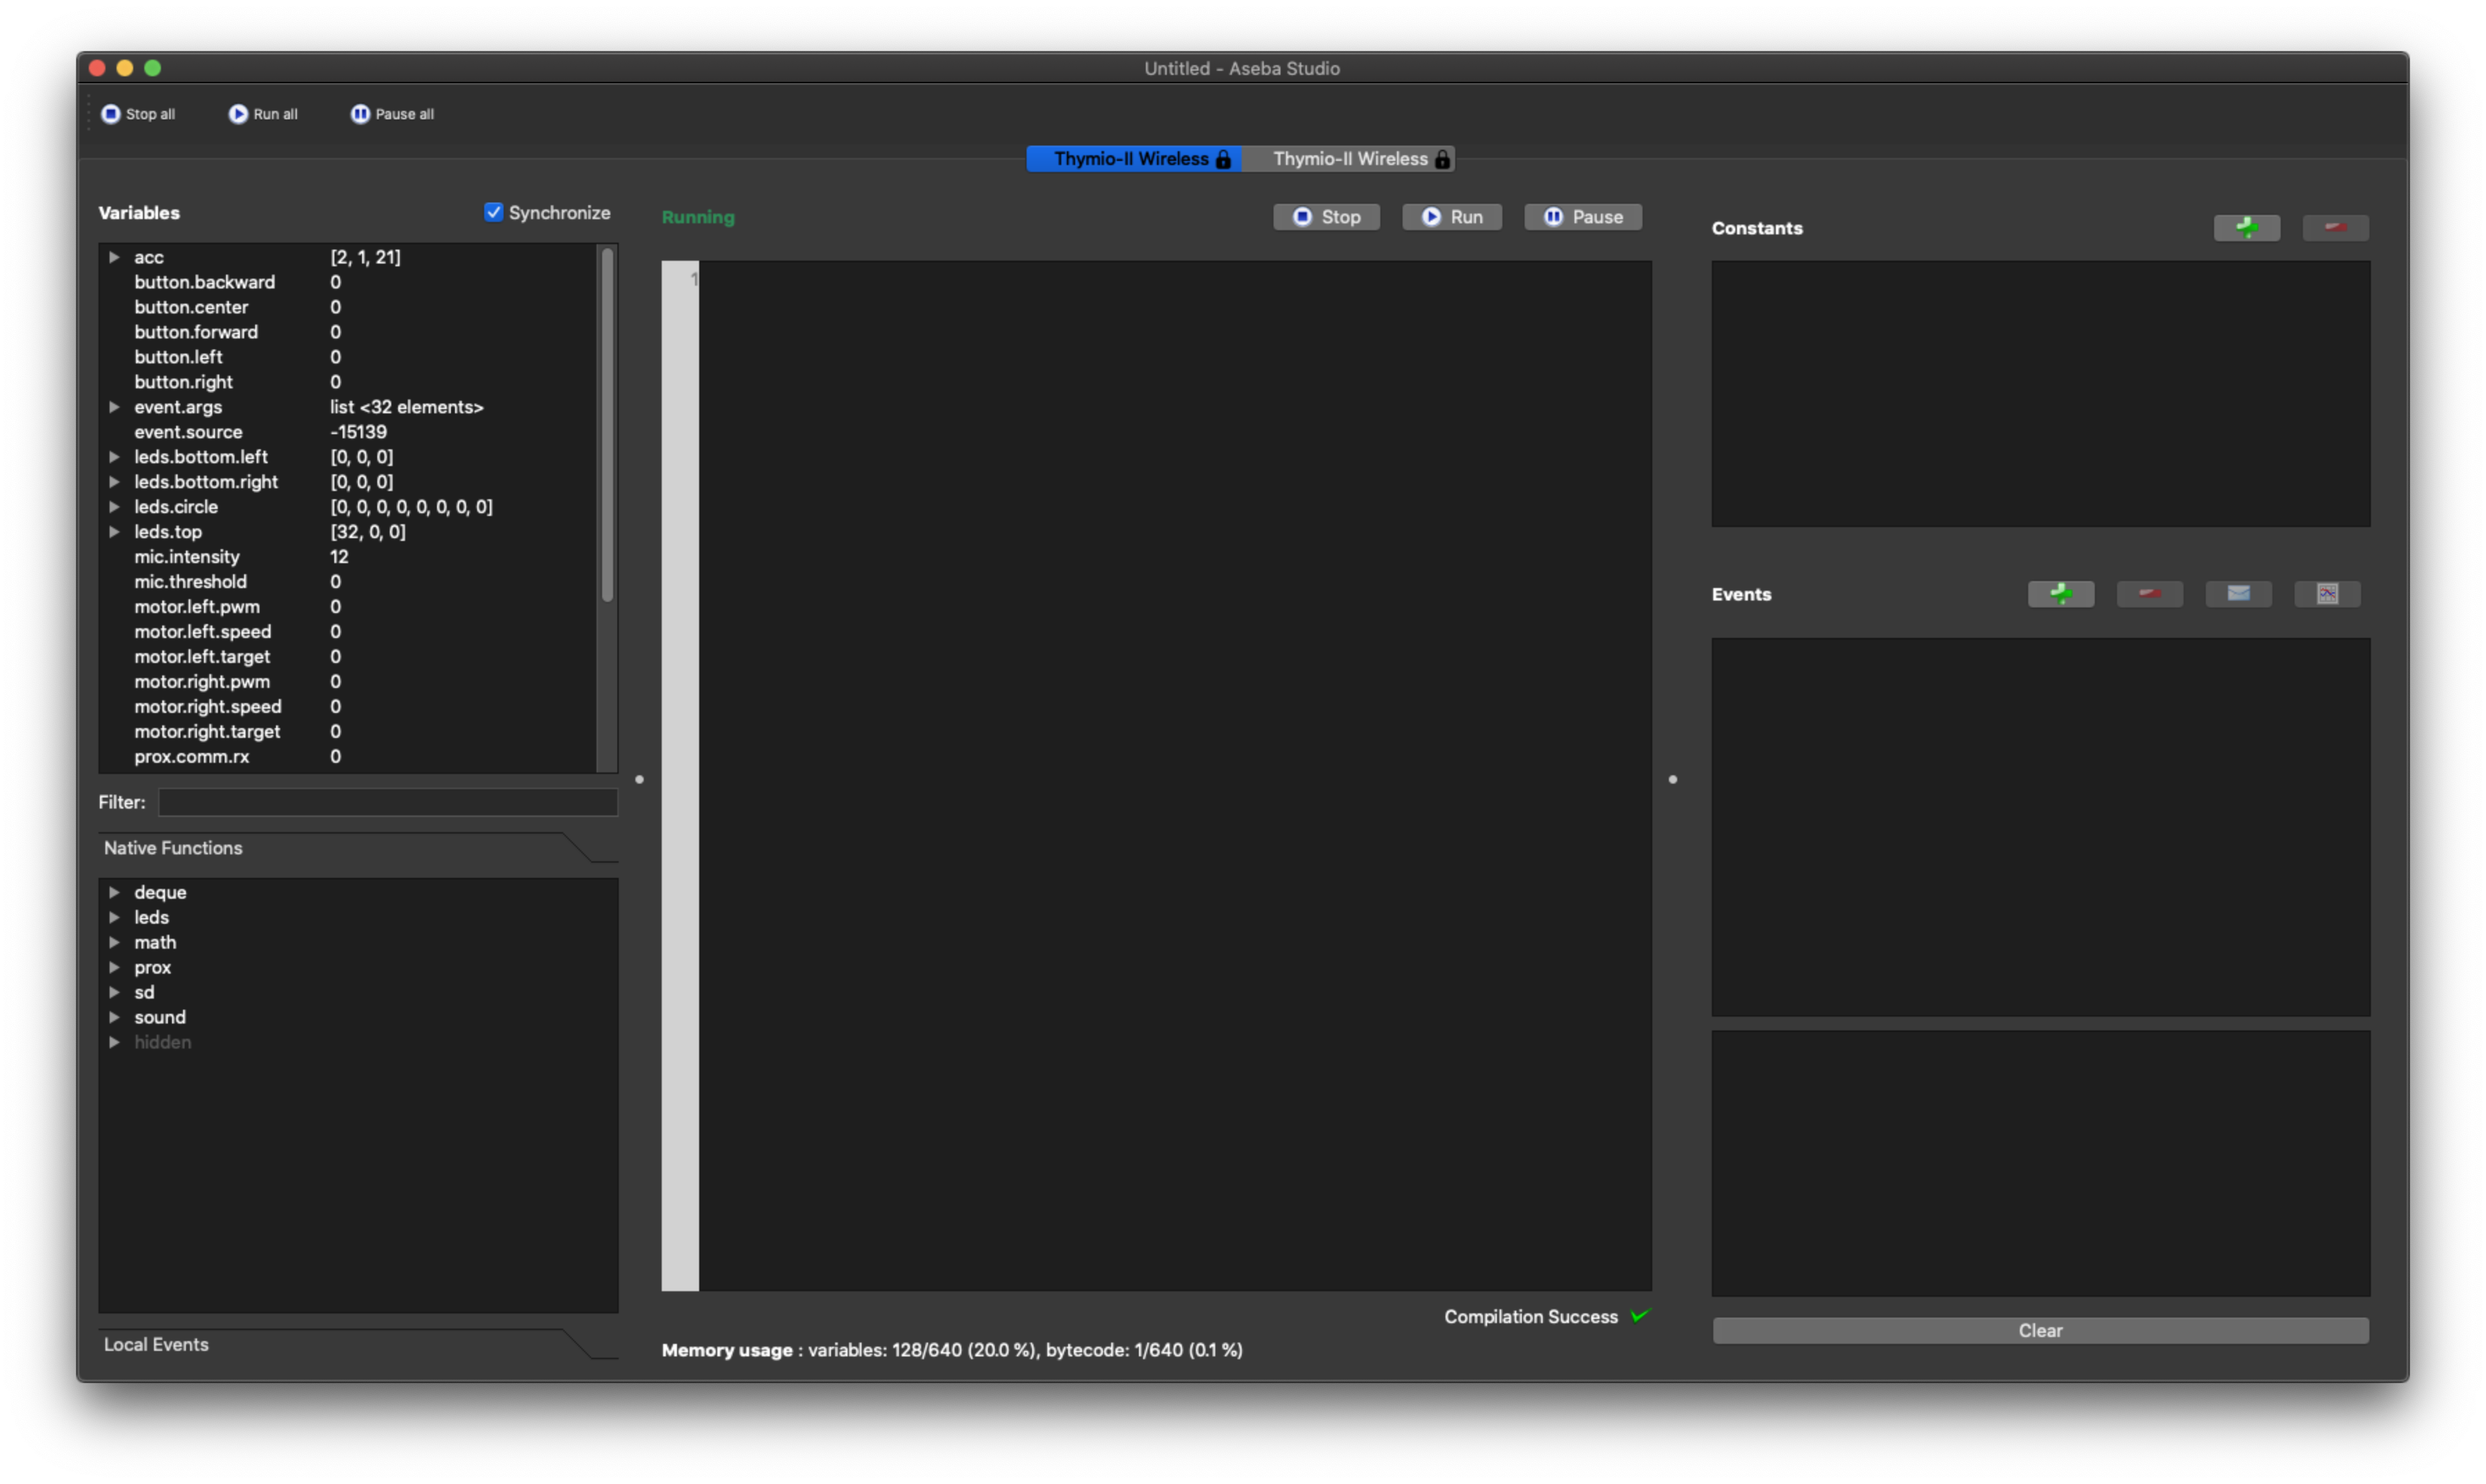
\includegraphics[width=\textwidth]{img/multiRobot.png}
	\caption{Aseba Studio con due robot collegati}
	\label{multiRobot}
\end{figure}

\newpage


\section{Comunicazione fra robot}\label{network}

È possibile far comunicare due robot tramite infrarossi (IR). Siccome la comunicazione avviene tramite i sensori orizzontali (cinque anteriori e due posteriori), i robot devono essere in grado di ``vedersi''.

Prima di tutto è necessario attivare la comunicazione IR su entrambi i robot, dopodiché si possono usare i blocchi o i comandi specialmente previsti (rispettivamente su Blockly e Aseba studio) per trasmettere e ricevere i segnali; purtroppo al momento questa funzione non è disponibile né in VPL né in Scratch.

Di seguito un semplice esempio dove il primo robot trasmette un segnale IR e il secondo reagisce cambiando il colore del LED superiore:

\begin{figure}[H]
	\centering
	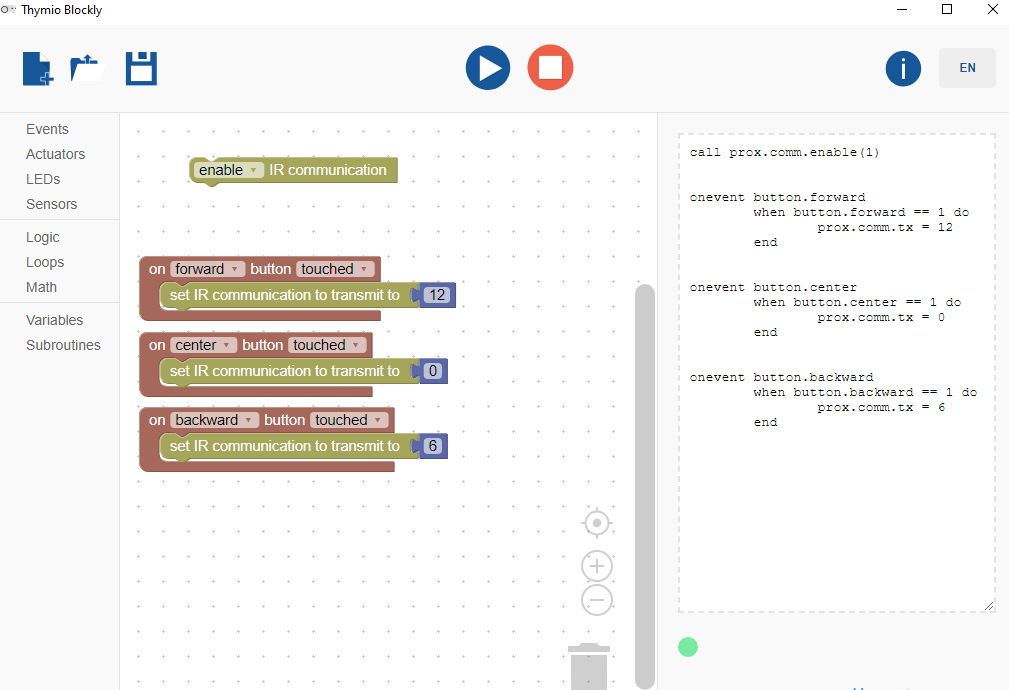
\includegraphics[width=0.9\textwidth]{img/blocklyIR1.png}
	\label{blocklyIR1}
\end{figure}

\begin{figure}[H]
	\centering
	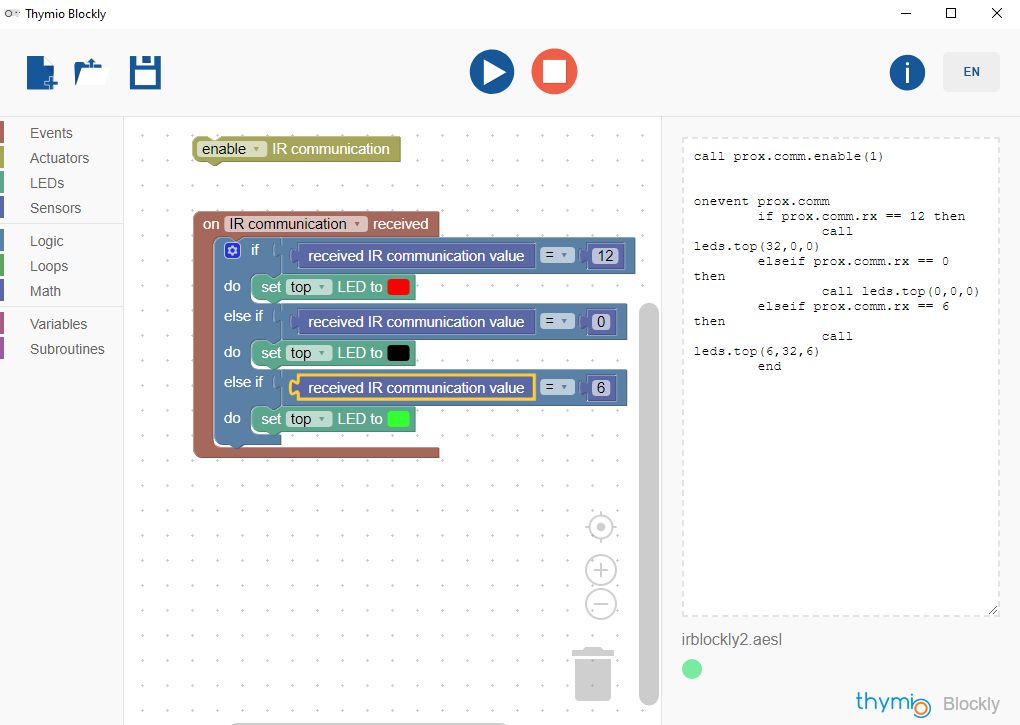
\includegraphics[width=0.9\textwidth]{img/blocklyIR2.png}
	\caption{Un semplice esempio di comunicazione fra due robot}
	\label{blocklyIR2}
\end{figure}


\section{Esempi di codice}\label{usiRepo}

Al seguente indirizzo sono disponibili diversi file con esempi di semplici programmi appositamente prodotti dall'USI:

\url{https://github.com/USI-Showroom/thymio/tree/master/examples}


- easyBlackLine: un semplice programma per far seguire a Thymio una linea nera con i due sensori inferiori

- IRcomm: semplice demo di come usare la comunicazione infrarossi fra due robot (vedi punto \ref{network}, richiede due robot)

- ledTest: accende tutti i LED presenti sul robot

- remoteDrive: un progetto per controllare il movimento di un Thymio tramite un altro (richiede due robot)

\newpage


\subsection{Risorse ufficiali}

Ai seguenti indirizzi sono disponibili diversi tutorial ed esempi ufficiali di codice:

\url{http://wiki.thymio.org/en:creations}

\url{https://github.com/Mobsya/thymio-programming-exercises}

\url{https://github.com/Mobsya/thymio-vpl-tutorial}


\end{document}
